\section{Motivation}
Modern day technology has developed under incredible speed in recent decade and the computing power growth rate is truly phenomenal and lasting impact can be felt and benefit us in many ways. It is important to realise the worldwide effect on environment by the increase in consumption of power by these technology advancements.

According to~\cite{pickavet2008worldwide}, the power consumption growth rates of PCs are about 7.5\% per year. Data Centres and network play much larger role as they both have power consumption rate of 12\% each. This considerable growth is due to increasing data to be accessed, stored and processed. This constant expansion of energy consumption leads to increase in carbon emissions. \(CO_2\) emissions from ICT (Information and communications technology) are increasing at a rate of 6\% per year, at such rate by 2020 it will account to 12\% of worldwide emissions ~\cite{rong2016optimizing}.

\begin{figure}[ht]
    \centering
    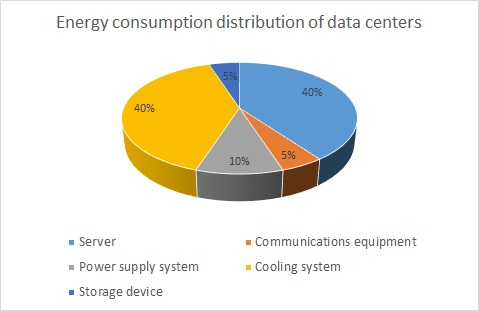
\includegraphics[width=200pt]{energypiechart}
    \caption{\label{fig:energypie} Energy consumption distribution of data centers.}    
\end{figure}

The major roles of power consumption by a data ware house is played by the servers and the cooling system which is used to cool down the server physical parts. From the figure~\ref{fig:energypie}, you can see they both account to 80\% of the total consumption with both accounting for 40\% each~\cite{rong2016optimizing}. Hence by finding a relation between different events and energy consumption, we could minimize the power consumption by the systems. Minimising energy consumed will also decrease the heat generated by the system which will in turn lower down the usage of cooling system. Leading us to minimise cost and save environment.

Thus, if we could discover the functional relational between the demand of the power and the performance events (PMCs), that could enable us the ability to adjust, and predict the energy consumption for certain computations.

Above is just only one field that possible usage of the functional relationship in data. In real world there are much more application that required such technique. Such as hybrid vehicle power management, power supply of auxiliary power units etc. There are many past work in this field but only few were focus on the relationship between dynamic energy consumption and PMCs. Hence, in this report we will try to observe the relationship between energy consumption and PMCs. We will explore the monotonicity of the relationship between dynamic energy consumption and performance events (PMCs) and suggesting the non-existence of a functional relationship as well.

\section{Approach}
Our main goal here is to find nonexistence of functional relationship. In other words, it means proving that the dataset cannot be explained in terms of a function/formula.

Our first approach to do so is to find two tuples such that \(n\) number of performance events are equal within some tolerance, but their dynamic energy consumption is the different. Existence of such a tuple in database will lead us to prove the non-existence of a functional relationship.

Second approach is to group \(n-1\) performance events and find dataset where the group size is greater than equal to three. In this approach we first assume here that the dataset provided has dynamic energy consumption equal to a linear combination of its performance events. Then using arithmetic, we compute the constant relating to the nth event. This constant will then be used to find the dynamic energy consumption of the third tuple in the group. If this test fails then we would be able to conclude the non-existence linear functional relation.

The third approach which follows the second is to operate on the existing records and make new records by simple addition as these performance events and consumption are additive in nature. And then on these new records, the first approach is run which means finding different dynamic energy consumption and validating the equality of the performance events associated with it.

The above three approaches help us to find the non-existence of linear relation or a functional relation. Our approaches are based on finding one irregularity which helps us to defy the assumptions that the dataset is linear or functional. This methodology does not prove or find the relationship. It rather defies the possibility of having one.

But we need to prove these approaches for the sake of our user to understand why the dataset cannot represented as a function. The proves for the above will be done in later chapter.

\section{Structure of report}
In this report, you must have already seen the motivation behind the project and brief description of the approaches that will be taken to reach the objective.

This Introductory chapter is followed by Background research, work done and work plan and the timeline of the project deliverables.

Background research explains about performance events and how do they influence energy consumption by the system. It shows some other reasons to test for functional relation. It explains the approaches mentioned above with proofs. So that one can be sure about the correctness of the program and understand the result. 

Following Background research is the work done. Work done contains simple observation that one found and analysis which will reflect the work plan. Work plan contains the timeline for the project. It lists out the deliverables of the project.